\section{Pianificazione}

\subsection{Modello di sviluppo}

Il modellosviluppo\textsubscript{G} scelto è il modello \textbf{incrementale}. Il modello incrementale\textsubscript{G} prevede che Analisi dei Requisiti e Progettazione Architetturale si svolgano una volta sola: queste attività\textsubscript{G} servono a studiare il problema e a strutturarne la soluzione. Si tornerà su queste attività\textsubscript{G} per eseguire incrementi mirati a raffinarne i contenuti in base a nuove evidenze individuate nei periodi successivi.

La progettazione di dettaglio e la codifica invece si svilupperanno attraverso cicli di incremento atti a integrare il sistema di nuove funzionalità: si partirà dal soddisfacimento dei requisito\textsubscript{G} obbligatori, per poi eventualmente incrementare con requisito\textsubscript{G} desiderabili e facoltativi. 

Queste modalità permettono, gettate le basi del prodotto, di accrescerne le funzionalità producendo valore fin da subito, in modo da avere riscontro quasi immediato sull'operato e poterne indirizzare gli sviluppi successivi in base ai feedback ricevuti, anche dal proponente, e alle risorsa\textsubscript{G} disponibili.

Il team adotterà anche alcune tecniche tipiche dello sviluppo Agile: viene fatto uso di una Kanban board, strumento che permette di pianificare in dettaglio e visualizzare gli obiettivi a cui ciascun membro del team si dedica. Questa tecnica riflette la modalità con cui il team si organizza nel contesto di un incremento: un meeting a cadenza settimanale permette di pianificare l'avanzamento e stabilire le future assegnazioni, in modo da affrontare eventuali ritardi o difficoltà prima che possano causare problemi allo sviluppo complessivo.



\subsection{Scadenze}

Il gruppo stabilisce di affrontare le revisione\textsubscript{G} di avanzamento nelle seguenti date:
\begin{itemize}
	\item \textbf{Revisione dei Requisiti}: 18 Gennaio 2021
	\item \textbf{Revisione di Progettazione}: 8 Marzo 2021 
	\item \textbf{Revisione di Qualifica}: 9 Aprile 2021
	\item \textbf{Revisione di Accettazione}: 10 Maggio 2021	
\end{itemize}





\subsection{Fasi}

A fronte del modellosviluppo\textsubscript{G} scelto e delle scadenze fissate, lo sviluppo procederà attraverso le seguenti fasi:
\begin{itemize}
	\item \textbf{Avvio}
	\item \textbf{Analisi dei Requisiti}
	\item \textbf{Progettazione Architetturale}
	\item \textbf{Progettazione di Dettaglio e Codifica dei Requisiti Obbligatori}
	\item \textbf{Progettazione di Dettaglio e Codifica dei Requisiti Desiderabili}
	\item \textbf{Validazione e Collaudo}
\end{itemize}


Nella settimana che intercorre tra la consegna degli artefatto\textsubscript{G} per la revisione\textsubscript{G} e la presentazione degli stessi, il gruppo è impegnato nelle seguenti attivita\textsubscript{G}: 
\begin{itemize}
	\item \textbf{Preparazione alla presentazione}: viene preparato il materiale necessario alla presentazione;
	\item \textbf{Verifica delle fase\textsubscript{G} precedenti}: il gruppo si vede coinvolto in un confronto dal quale vorranno emergere le criticità riscontrate nelle fase\textsubscript{G} trascorse dall'ultima revisione\textsubscript{G}, al fine di migliorare lo svolgimento delle fase\textsubscript{G} successive;
	\item \textbf{Approfondimento personale}: ogni membro del gruppo spende alcune ore per formare e consolidare una conoscenza di base degli strumenti e tecniche da impiegare nella fase\textsubscript{G} successiva.
\end{itemize}
Queste attivita\textsubscript{G} non verranno esplicitate nella descrizione di dettaglio che segue, in quanto ripetitive.



\subsubsection{Avvio}

\textit{Dal 2020-11-12 al 2020-12-13}
\\\\
Questa fase\textsubscript{G} inizia in corrispondenza del primo seminario tecnologico tenuto da una delle aziende proponenti e termina con la scelta del capitolato\textsubscript{G} a cui il gruppo intende avanzare la propria offerta nella relativa gara d'appalto.
In questa fase\textsubscript{G} vengono svolte le seguenti attivita\textsubscript{G}:
\begin{itemize}
	\item \textbf{Visione dei Seminari}: i seminari tecnologici costituiscono un fattore importante nel contesto della scelta del capitolato\textsubscript{G}, fanno luce sui requisito\textsubscript{G} e sulla fattibilità dei progetto\textsubscript{G};
	\item \textbf{Setup Strumenti}: inizia in questa fase\textsubscript{G} la definizione delle norme che il gruppo intende adottare. Si studiano e testano gli strumenti che permetteranno l'organizzazione interna, il tracciamento, la stesura dei documenti e il loro versionamento, la gestione dei meeting e la loro calendarizzazione. L'Amministratore è la figura che principalmente si fa carico di questi oneri;
	\item \textbf{Studio di Fattibilità}: l'analisi del materiale di ogni capitolato\textsubscript{G} permette al gruppo di farsi una prima idea sui punti di forza e sulle criticità di ognuno. Terminata la visione dei seminari, si effettua uno studio approfondito di ogni progetto\textsubscript{G} e gli Analisti redigono lo \textsc{Studio di Fattibilità}, nel quale viene espressa la preferenza definitiva;
	\item \textbf{Piano di Progetto}: il Responsabile di Progetto inizia la redazione del \textsc{Piano di Progetto} nelle sue parti fondamentali, a partire da una prima definizione delle fase\textsubscript{G} e dei rischi.
\end{itemize}  


\begin{figure}[H]
	\centering
	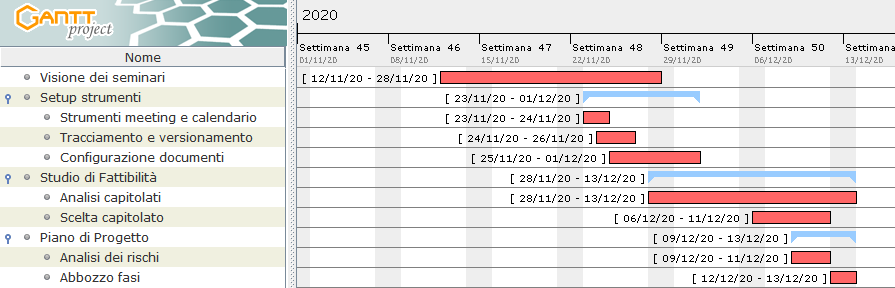
\includegraphics[scale=0.62]{res/images/01_gantt_avvio.png}
	\caption{Diagramma di gantt\textsubscript{G} relativo alla fase\textsubscript{G} di Avvio}
\end{figure}




\subsubsection{Analisi dei Requisiti}

\textit{Dal 2020-12-13 al 2021-01-11}
\\\\
Questa fase\textsubscript{G} inizia al termine della fase\textsubscript{G} di Avvio e si conclude con la consegna dei documenti per la Revisione dei Requisiti.
In questa fase\textsubscript{G} vengono svolte le seguenti attivita\textsubscript{G}:
\begin{itemize}
	\item \textbf{Studio di Fattibilità}: si verifica lo \textsc{Studio di Fattibilità} redatto durante la fase\textsubscript{G} di Avvio;
	\item \textbf{Norme di Progetto}: vengono stabilite le norme di progetto\textsubscript{G} pianificando nel dettaglio i processi primari, i processi di sviluppo e i processi organizzativi. Il documento \textsc{Norme di Progetto} viene redatto dall'Amministratore;
	\item \textbf{Piano di Progetto}: il Responsabile di Progetto redige il \textsc{Piano di Progetto} scandendo le fase\textsubscript{G} secondo cui si articolerà il lavoro, presentando il preventivo dei periodo\textsubscript{G} e il consuntivo delle prime 2 fase\textsubscript{G};
	\item \textbf{Analisi dei Requisiti}: gli Analisti effettuano uno studio approfondito del capitolato\textsubscript{G} e ne individuano i requisito\textsubscript{G}: l'analisi si caratterizza da contatti frequenti con il proponente che fornirà supporto nella comprensione del problema. Viene completata la redazione dell'\textsc{Analisi dei Requisiti} da parte degli Analisti. Quest'attività è bloccante per la prosecuzione del progetto\textsubscript{G};
	\item \textbf{Piano di Qualifica}: in questa attivita\textsubscript{G} si individuano i criteri che garantiscono la qualità del prodotto. Il \textsc{Piano di Qualifica} è redatto dai Verificatori;
	\item \textbf{Glossario}: il \textsc{Glossario} conterrà i termini a cui si riterrà necessario dare definizione. La stesura avviene da parte degli Analisti;
	\item \textbf{Verifica dei documenti}: quest'attività si concentra nella settimana che precede la presentazione e ha l'obiettivo di verificare e certificare la qualità di tutti i documenti prodotti. I Verificatori sono i protagonisti di quest'attività;
	\item \textbf{Lettera di Presentazione}: avviene la stesura della lettera con cui il gruppo si candida alla Revisione dei Requisiti. La sua preparazione e consegna è in carico al Responsabile.
\end{itemize}

\begin{figure}[H]
	\centering
	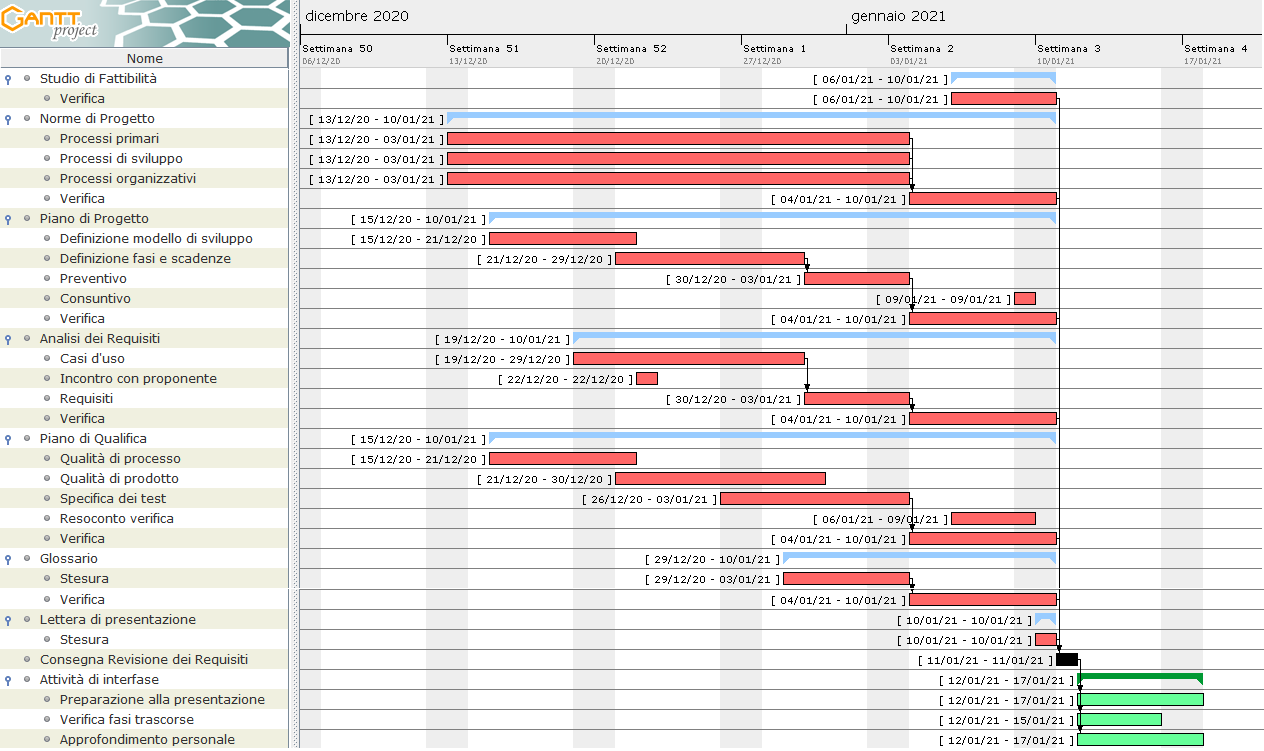
\includegraphics[scale=0.45]{res/images/02_gantt_analisi_requisiti.png}
	\caption{Diagramma di gantt\textsubscript{G} relativo alla fase\textsubscript{G} di Analisi dei Requisiti}
\end{figure}


\subsubsection{Progettazione Architetturale}

\textit{Dal 2021-01-18 al 2021-03-01}
\\\\
Inizia il giorno successivo alla presentazione della Revisione dei Requisiti e termina in corrispondenza della consegna degli artefatto\textsubscript{G} per la Revisione di Progettazione.
\begin{itemize}
	\item \textbf{Allegato Tecnico}: viene redatto l'\textsc{Allegato Tecnico}, nel quale viene presentata la Technology Baseline, ovvero l'architettura ad alto livello del software. Redatto dai Progettisti;
	\item \textbf{Proof of Concept}: una prima implementazione della soluzione permette di valutarne la bontà: viene realizzato un prototipo del software da parte dei Programmatori;
	\item \textbf{Incremento e Verifica della Documentazione}: l'avanzamento nello sviluppo del prodotto chiarirà alcuni aspetti che nella fase\textsubscript{G} di Analisi risultavano oscuri, e potrebbe evidenziare delle criticità non inizialmente considerate. Se necessario, viene raffinata l'\textsc{Analisi dei Requisiti}. Anche il \textsc{Piano di Progetto} viene migliorato fornendo maggior dettaglio, oltre che integrato con il consuntivo della fase\textsubscript{G} trascorsa. Le \textsc{Norme di Progetto} riguardano ora anche gli strumenti necessari alla progettazione architetturale, e il \textsc{Glossario} si vede integrato con nuovi termini. Il \textsc{Piano di Qualifica} prevede ora anche i criteri di qualità per la progettazione. Generali miglioramenti sono apportati in base alle indicazioni ricevute con la Revisione dei Requisiti. L'integrazione avviene ad opera delle figure interessate alla stesura dei documenti nelle fase\textsubscript{G} precedenti;
	\item \textbf{Lettera di Presentazione}: avviene la stesura della lettera con cui il gruppo si candida alla Revisione di Progettazione. La sua preparazione e consegna è in carico al Responsabile.
\end{itemize}

\begin{figure}[H]
	\centering
	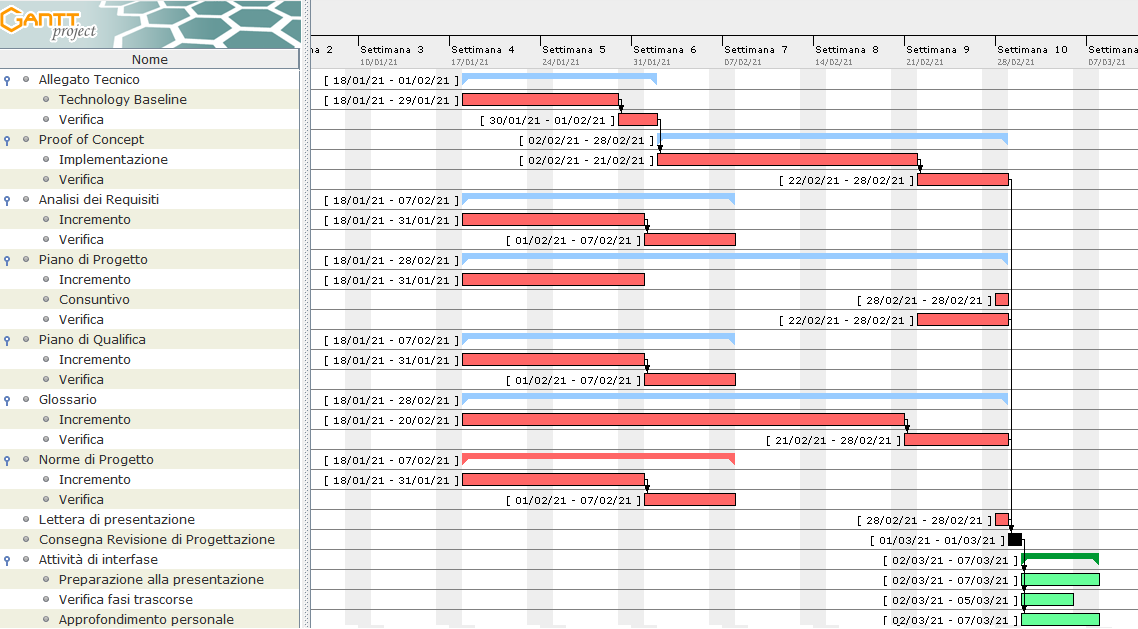
\includegraphics[scale=0.50]{res/images/03_gantt_progettazione.png}
	\caption{Diagramma di gantt\textsubscript{G} relativo alla fase\textsubscript{G} di Progettazione Architetturale}
\end{figure}

\subsubsection{Progettazione di Dettaglio e Codifica dei Requisiti Obbligatori}

\textit{Dal 2021-03-08 al 2021-03-21}
\\\\
Inizia il giorno successivo alla presentazione della Revisione di Progettazione e si conclude con la presentazione della Product Baseline \footnote{Questa milestone\textsubscript{G} può coincidere con la consegna degli artefatto\textsubscript{G} per la Revisione di Qualifica nel caso in cui non vi siano sufficienti risorsa\textsubscript{G} per procedere con il soddisfacimento dei requisito\textsubscript{G} desiderabili.
\begin{itemize}
	\item \textbf{Allegato Tecnico}: viene integrato l'\textsc{Allegato Tecnico}, che presenterà ora anche la Product Baseline, nella quale il software è scomposto e analizzato nelle sue unità. Redatto dai Progettisti e dai Programmatori;
	\item \textbf{Codifica}: la scrittura del codice ad opera dei Programmatori segue i criteri di qualità stabiliti nel \textsc{Piano di Qualifica} e riguarda i soli requisito\textsubscript{G} obbligatori. Il codice prodotto viene poi verificato;
	\item \textbf{Incremento e Verifica della Documentazione}: se necessario, viene raffinata l'\textsc{Analisi dei Requisiti}. Il \textsc{Piano di Progetto} viene integrato con il consuntivo della fase\textsubscript{G} trascorsa.  Le \textsc{Norme di Progetto} riguardano ora anche gli strumenti necessari alla codifica, e il \textsc{Glossario} comprende nuovi termini. Il \textsc{Piano di Qualifica} prevede ora anche i criteri di qualità per la codifica. Generali miglioramenti sono apportati in base alle indicazioni ricevute con la Revisione di Progettazione. L'integrazione avviene ad opera delle figure interessate alla stesura dei documenti nelle fase\textsubscript{G} precedenti.
	
\end{itemize}


\begin{figure}[H]
	\centering
	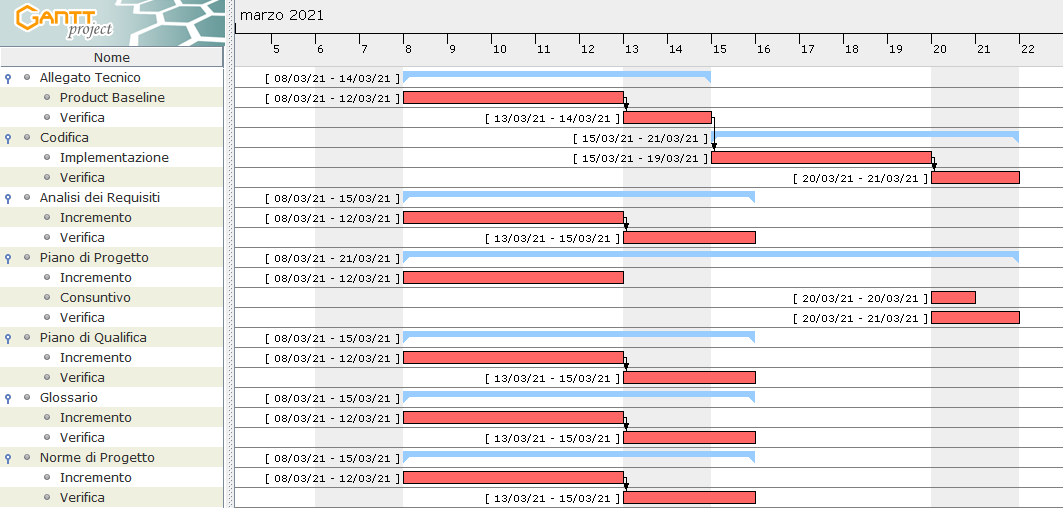
\includegraphics[scale=0.52]{res/images/04_gantt_codifica_obbligatori.png}
	\caption{Diagramma di gantt\textsubscript{G} relativo alla fase\textsubscript{G} di Progettazione  e Codifica dei Requisiti Obbligatori}
\end{figure}



\subsubsection{Progettazione di Dettaglio e Codifica dei Requisiti Desiderabili e Facoltativi}

\textit{Dal 2021-03-22 al 2021-04-02}
\\\\
Inizia il giorno successivo alla presentazione della Product Baseline e termina in corrispondenza della consegna degli artefatto\textsubscript{G} per la Revisione di Qualifica \footnote{Questa fase\textsubscript{G} potrebbe non essere svolta se le risorsa\textsubscript{G} dovessero non risultare sufficienti a soddisfare i requisito\textsubscript{G} desiderabili e facoltativi. In questo caso verrà comunque redatta la \textsc{Lettera di Presentazione} e registrato il bilancio consuntivo.}.
\begin{itemize}
	\item \textbf{Codifica}: la scrittura del codice ad opera dei Programmatori segue i criteri di qualità stabiliti nel \textsc{Piano di Qualifica} e riguarda ora i requisito\textsubscript{G} desiderabili. Il codice prodotto viene poi verificato;
	\item \textbf{Allegato Tecnico}: la Product Baseline viene incrementata per includere i requisito\textsubscript{G} desiderabili e quelli facoltativi;
	\item \textbf{Incremento e Verifica della Documentazione}: se necessario, viene raffinata l'\textsc{Analisi dei Requisiti}. Il \textsc{Piano di Progetto} viene integrato con il consuntivo della fase\textsubscript{G} trascorsa. L'integrazione avviene ad opera delle figure interessate alla stesura dei documenti nelle fase\textsubscript{G} precedenti;
	\item \textbf{Lettera di Presentazione}: avviene la stesura della lettera con cui il gruppo si candida alla Revisione di Qualifica. La sua preparazione e consegna è in carico al Responsabile.
	
\end{itemize}


\begin{figure}[H]
	\centering
	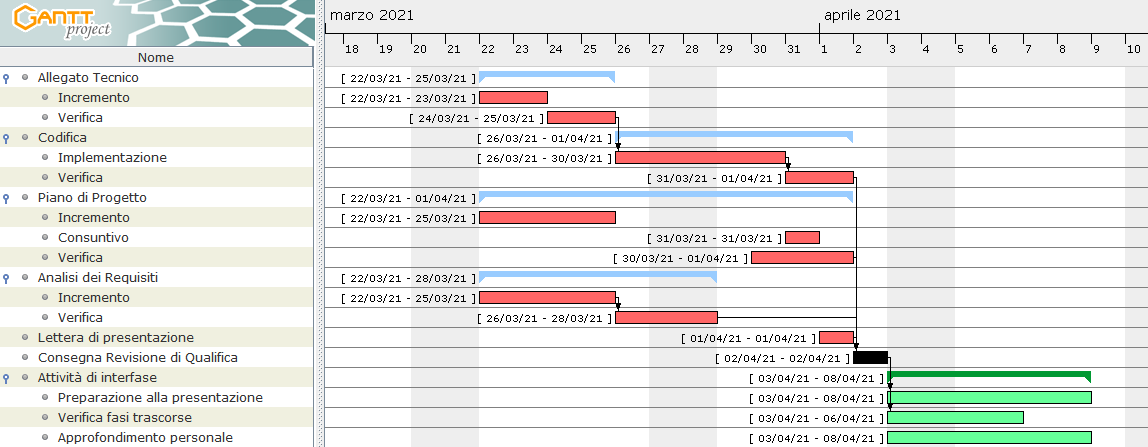
\includegraphics[scale=0.48]{res/images/05_gantt_codifica_desiderabili.png}
	\caption{Diagramma di gantt\textsubscript{G} relativo alla fase\textsubscript{G} di Progettazione e Codifica dei Requisiti Desiderabili e Facoltativi}
\end{figure}



\subsubsection{Validazione e Collaudo}

\textit{Dal 2021-04-09 al 2021-05-03}
\\\\
Inizia il giorno successivo alla presentazione della Revisione di Qualifica e termina in corrispondenza della consegna degli artefatto\textsubscript{G} per la Revisione di Accettazione.
\begin{itemize}
	\item \textbf{Validazione e Collaudo}: vengono eseguiti ulteriori test per consolidare e garantire la qualità del prodotto. Il \textsc{Piano di Qualifica} è il documento di riferimento per quest'attività. \`E svolta dai Progettisti e dai Programmatori;
	\item \textbf{Manuale Utente}: il \textsc{Manuale Utente}, la cui stesura è affidata ai Progettisti e agli Analisti, specifica le modalità d'uso del software agli utenti utilizzatori;
	\item \textbf{Incremento e Verifica della Documentazione}: il \textsc{Piano di Progetto} viene integrato con il consuntivo della fase\textsubscript{G} trascorsa. Generali miglioramenti sono apportati in base alle indicazioni ricevute con la Revisione di Qualifica. L'integrazione avviene ad opera delle figure interessate alla stesura dei documenti nelle fase\textsubscript{G} precedenti;
	\item \textbf{Lettera di Presentazione}: avviene la stesura della lettera con cui il gruppo si candida alla Revisione di Accettazione. La sua preparazione e consegna è in carico al Responsabile.
\end{itemize}

\begin{figure}[H]
	\centering
	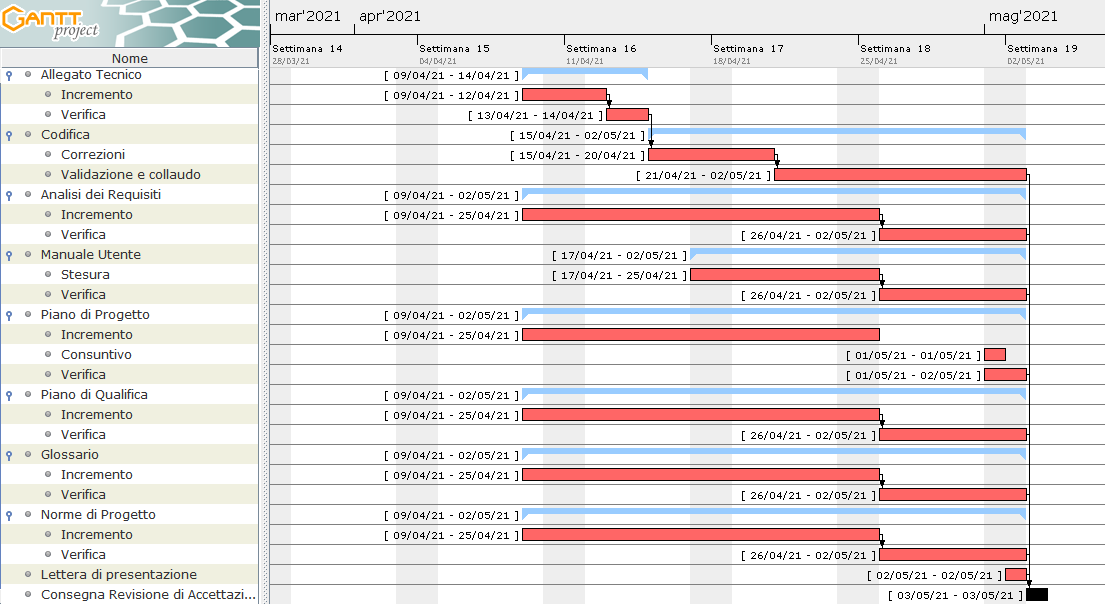
\includegraphics[scale=0.51]{res/images/06_gantt_validazione}
	\caption{Diagramma di gantt\textsubscript{G} relativo alla fase\textsubscript{G} di Validazione e Collaudo}
\end{figure}